
%\renewcommand{\theequation}{\theenumi}
%\begin{enumerate}[label=\arabic*.,ref=\thesubsection.\theenumi]
%\numberwithin{equation}{enumi}

\item A=$[a_{ij}]_{mxn}$ is a square matrix,if\\
(A) m$<$n (B)m$>$n (C) m=n (D) None of these\\
\item Which of the given values of x and y make the following pair of matrices equal \myvec{3x+7 &5\\y+1 &2-3x},\myvec{0 &y-2\\8 &4}\\
(A)x=$\frac{-1}{3}$,y=7 \\
 (B) Not possible to find\\
(C) y=7, x=$\frac{-2}{3}$\\
 (D) x=$\frac{-1}{3}$,y=$\frac{-2}{3}$\\
\item The number of all possible matrices of order 3X3 with each entry 0 or 1 is:\\
(A) 27 (B)18 (C)81 (D)512\\
\item Let A=\myvec{2 &4\\3 &2},B=\myvec{1 &3\\-2 &5},C=\myvec{-2 &5\\3 &4}
Find each of the following:\\
(i) A+B  (ii)A-B  (iii)3A-C  (iv)AB  (v)BA\\
\solution
\begin{enumerate}
  \item 
  \item 
  \item \begin{align}
    \vec{A}-\vec{B}     = \myvec{1&1\\5&-3}
\end{align}

  \item \begin{align}
    \vec{A}-\vec{B}     = \myvec{1&1\\5&-3}
\end{align}

\end{enumerate}
\item Compute the following:\\
(i)\myvec{a &b\\-b &a}+\myvec{a &b\\b&a} (ii)\myvec{a^2+b^2 &b^2+c^2\\a^2+c^2 &a^2+b^2}+\myvec{2ab &2bc\\-2ac &-2ab} \\
  (iii) \myvec{-1 &4 &-6\\8 &5 &16\\2 &8 &5}+\myvec{12 &7 &6\\8 &0 &5\\3 &2 &4}\\ 
(iv) \myvec{cos^2x &sin^2x\\sin^2x &cos^2x}+\myvec{sin^2x &cos^2x\\cos^2x &sin^2x}\\
\item Compute the indicated products.
\begin{enumerate}
\item \myvec{2 &3 &4\\3 &4 &5\\4 &5 &6}\myvec{1 &-3 &5\\0 &2 &4\\3 &0 &5} 
\item \myvec{2 &1\\3 &2\\-1 &1}\myvec{1 &0 &1\\-1 &2 &1} \\
\item  \myvec{3 &-1 &3\\-1 &0 &2}\myvec{2 &-3\\1 &0\\3 &1}
\end{enumerate}
\solution
\begin{enumerate}
\item \begin{align}
    \vec{A}-\vec{B}     = \myvec{1&1\\5&-3}
\end{align}

\end{enumerate}
\item If,A=\myvec{1 &2 &-3\\5 &0 &2\\1 &-1 &1},B=\myvec{3 &-1 &2\\4 &2 &5\\2 &0 &3}and C=\myvec{4 &1 &2\\0 &3 &2\\1 &-2 &3},then compute (A+B) and (B-C).Also ,verify that A+(B-C)=(A+B)-C.\\
\solution
\begin{align}
    \vec{A+B}&=\myvec{1&2&-3\\5&0&2\\1&-1&1}+\myvec{3&-1&2\\4&2&5\\2&0&3}\\
    &=\myvec{1+3&2+(-1)&-3+2\\5+4&0+2&2+5\\1+2&-1+0&1+3}\\
    &=\myvec{4&1&-1\\9&2&7\\3&-1&4}
 \end{align}
 \begin{align}
     \vec{B-C}&=\myvec{3&-1&2\\4&2&5\\2&0&3}-\myvec{4&1&2\\0&3&2\\1&-2&3}\\
     &=\myvec{3-4&-1-1&2-2\\4-0&2-3&5-2\\2-1&0-(-2)&3-3}\\
     &=\myvec{-1&-2&0\\4&-1&3\\1&2&0}
 \end{align}
 \begin{align}
     \vec{A}+\brak{\vec{B-C}}&=\myvec{1&2&-3\\5&0&2\\1&-1&1}+\myvec{-1&-2&0\\4&-1&3\\1&2&0}\\
     &=\myvec{1+(-1)&2+(-2)&-3+0\\5+4&0+(-1)&2+3\\1+1&-1+2&1+0}\\
     &=\myvec{0&0&-3\\9&-1&5\\2&1&1}\label{aug/2/7/2.0.9}
 \end{align}
 \begin{align}
     \brak{\vec{A+B}}-\vec{C}&=\myvec{4&1&-1\\9&2&7\\3&-1&4}-\myvec{4&1&2\\0&3&2\\1&-2&3}\\
     &=\myvec{4-4&1-1&-1-2\\9-0&2-3&7-2\\3-1&-1-(-2)&4-3}\\
     &=\myvec{0&0&-3\\9&-1&5\\2&1&1}\label{aug/2/7/2.0.12}
 \end{align}
 \eqref{aug/2/7/2.0.9} is same as \eqref{aug/2/7/2.0.12}
 
\item If A=$\myvec{\frac{2}{3} & 1 & \frac{5}{3}\\ \frac{1}{3} & \frac{2}{3} & \frac{4}{3} \\ \frac{7}{3} &2  & \frac{2}{3}}$ and B=$\myvec{\frac{2}{5} & \frac{3}{5} &1 \\ \frac{1}{5} & \frac{2}{5} & \frac{4}{5}\\ \frac{7}{5} & \frac{6}{5} & \frac{2}{5}}$,then compute 3A-5B.\\

\item Find x and y,if 2 \myvec{1 &3\\0 &x}+\myvec{y &0\\1 &2}=\myvec{5 &6\\1 &8}\\
\solution
\begin{align}
    2\myvec{1&3\\0&x} + \myvec{y&0\\1&2} &= \myvec{5&6\\1&8}\\
    \implies \myvec{2&6\\0&2x} + \myvec{y&0\\1&2} &= \myvec{5&6\\1&8}\\
    \implies \myvec{2+y&6+0\\0+1&2x+2} &= \myvec{5&6\\1&8}\\
    \implies 2+y=5,\; 2x&+2=8\\
    \implies y=3,\; x&=3
\end{align}
\item Solve the equation for x,y,z and t,if \\
2\myvec{x &z\\y &t}+3\myvec{1 &-1\\0 &2}=3\myvec{3 &5\\4 &6}\\
\item If x=\myvec{2 \\3}+y\myvec{-1 \\1}=\myvec{10 \\5},find the values of x and y.\\
\solution

\begin{equation}
    \vec{B} - \vec{A} = \myvec{-3\\-5\\-3}, \vec{C} - \vec{A} = \myvec{3\\5\\13}
\end{equation}
Forming the matrix 
\begin{align}
    \vec{M} &= \myvec{
    \vec{B} -  \vec{A} & \vec{C} - \vec{A}\\
    }^\top\\
    &= \myvec{
    -3 & -5 & -3\\
    3 & 5 & 3}
\end{align}
Using matrix transformation,
\begin{align}
 \vec{M} = \myvec{
    -3 & -5 & -3\\
    3 & 5 & 3}
    \xleftrightarrow{\text{$R_2$}\rightarrow{\text{$R_2 + R_1$ }}}
 \myvec{
 -3 & -5 & -3\\
 0 & 0 & 0}\
\end{align}
\begin{equation}
   \implies rank(\vec{M}) = 1 
\end{equation}
Thus $\vec{A}$, $\vec{B}$ and $\vec{C}$ are collinear.
% \begin{figure}[!h]
%          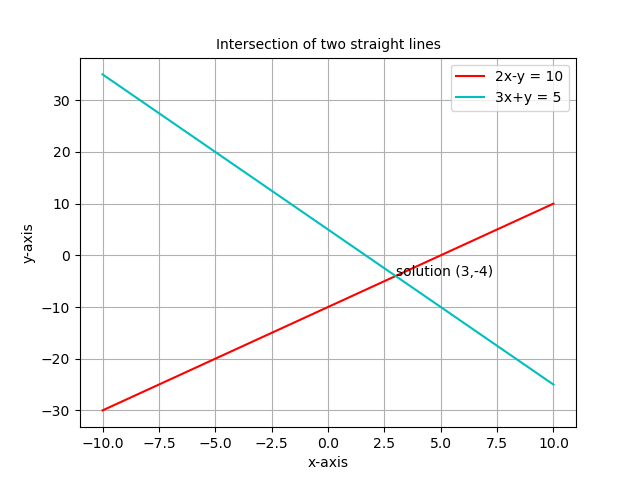
\includegraphics[width=\columnwidth]{solutions/aug/2/14/Figures/plot.png}
%          \caption{Plot of the line}
% \end{figure}

\item Given 3\myvec{x &y\\z &w}=\myvec{x &6\\-1 &2w}+\myvec{4 &x+y\\z+w &3},find the values of x,y,z and w.\\


Assume X,Y,Z,W and P are matrices of orders $2\times n$,$3 \times k$,$2\times p$,$n\times 3$ and $p\times k$,respectively.\\
Choose the correct answer in Exercise 31 and 32.\\
\item The restriction on n,k and p so that PY+WY will be defined are:\\
(A)k=3,p=n\\
 (B)k is arbitrary,p=2 \\
 (C)p is arbitrary,k=3 \\
 (D)k=2,p=3\\
\item If n=p,then the order of the matrix 7X-5Z is:\\
(A)$p \times 2$ (B)$2 \times n$ (C)$n \times 3$ (D)$p \times n$\\
\item Find the transpose of each of the following matrices:\\
(i)\myvec{5\\ \frac{1}{2} \\-1}\\ (ii)\myvec{1 &-1\\2 &3}\\ (iii)\myvec{-1 &5 &6\\\sqrt{3} &5 &6\\2 &3 &-1}\\
\item If A=\myvec{-1 &2 &3\\5 &7 &9\\-1 &1 &1} and B=\myvec{-4 &1 &-5\\1 &2 &0\\1 &3 &1},then verify that\\
(i)$(A+B)^{'}=A^{'}+B^{'}$ \\(ii) $(A-B)^{'}=A^{'}-B^{'}$\\
\solution
\begin{enumerate}
  \item 
  \item 


We clearly have,
\begin{align}
\vec{A}-\vec{B} =
\myvec{
3 & 1 & 8\\
4 & 5 & 9\\
-2 & -2 & 0}
\end{align}
Therefore 
\begin{align}
(\vec{A}-\vec{B})^\top =
\myvec{
3 & 4 & -2\\
1 & 5 & -2\\
8 & 9 & 0}\label{aug/2/16/2eq:1}
\end{align}
Now,
\begin{align}
\vec{A}^\top-\vec{B}^\top &=
\myvec{
-1 & 5 & -1\\
2 & 7 & 1\\
3 & 9 & 1}-
\myvec{
-4 & 1 & 1\\
1 & 2 & 3\\
-5 & 0 & 1}\\
\vec{A}^\top-\vec{B}^\top &=
\myvec{
3 & 4 & -2\\
1 & 5 & -2\\
8 & 9 & 0}\label{aug/2/16/2eq:2}
\end{align}
Therefore from \eqref{aug/2/16/2eq:1} and \eqref{aug/2/16/2eq:2} we can conclude that $(\vec{A}-\vec{B})^\top = \vec{A}^\top-\vec{B}^\top$.





\end{enumerate}
\item If $A^{'}$=\myvec{3 &4\\-1 &2\\0 &1} and B=\myvec{-1 &2 &1\\1 &2 &3},then verify that\\
(i) $(A+B)^{'}=A^{'}+B^{'}$ (ii)$(A-B)^{'}=A^{'}-B^{'}$
\\
\solution
\begin{enumerate}
  \item 
\begin{equation}
    \vec{B} - \vec{A} = \myvec{-3\\-5\\-3}, \vec{C} - \vec{A} = \myvec{3\\5\\13}
\end{equation}
Forming the matrix 
\begin{align}
    \vec{M} &= \myvec{
    \vec{B} -  \vec{A} & \vec{C} - \vec{A}\\
    }^\top\\
    &= \myvec{
    -3 & -5 & -3\\
    3 & 5 & 3}
\end{align}
Using matrix transformation,
\begin{align}
 \vec{M} = \myvec{
    -3 & -5 & -3\\
    3 & 5 & 3}
    \xleftrightarrow{\text{$R_2$}\rightarrow{\text{$R_2 + R_1$ }}}
 \myvec{
 -3 & -5 & -3\\
 0 & 0 & 0}\
\end{align}
\begin{equation}
   \implies rank(\vec{M}) = 1 
\end{equation}
Thus $\vec{A}$, $\vec{B}$ and $\vec{C}$ are collinear.
% \begin{figure}[!h]
%          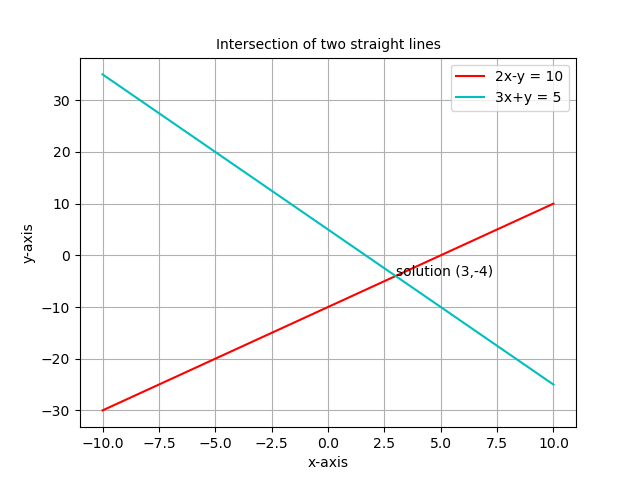
\includegraphics[width=\columnwidth]{solutions/aug/2/14/Figures/plot.png}
%          \caption{Plot of the line}
% \end{figure}

  \item 
\end{enumerate}

\item If$ A^{'}$=\myvec{-2 &3\\1 &2} and B=\myvec{-1 &0\\1 &2},then find that $(A+2B)^{'}$\\

  \item (i) Show that the matrix A=\myvec{1 &-1&5\\-1 &2 &1\\5 &1 &3} is a symmetric matrix.\\
  (ii) Show that the matrix A=\myvec{0 & 1 &-1\\-1 &0 &1\\1&-1 &0} is a skew symmetric matrix.\\
  \solution
  \begin{enumerate}
    \item Given,
    \begin{align}
    \label{aug/2/19/eq:1}
        \vec{A}=\myvec{1 & -1 & 5\\ -1 & 2 & 1\\5 & 1 & 3}
    \end{align}
    Transposing the matrix,
    \begin{align}
        \label{aug/2/19/eq:2}
        \vec{A}^\top=\myvec{1 & -1 & 5 \\-1 & 2 & 1\\5 & 1 &3}
    \end{align}
    Using \eqref{aug/2/19/eq:1} and \eqref{aug/2/19/eq:2} we get,
    \begin{align}
        \vec{A}=\vec{A}^\top
    \end{align}
    %\begin{center}
        $\therefore \vec{A}$ is symmetric matrix. 
    %\end{center}
        
    \item Given,
    \begin{align}
    \label{aug/2/19/eq:4}
        \vec{A}=\myvec{0 & 1 & -1\\ -1 & 0 & 1\\1 & -1 & 0}
    \end{align}
    Transposing the matrix,
    \begin{align}
        \label{aug/2/19/eq:5}
        \vec{A}^\top=\myvec{0 & -1 & 1 \\1 & 0 & -1\\-1 & 1 & 0}
    \end{align}
    Using \eqref{aug/2/19/eq:4} and \eqref{aug/2/19/eq:5} we get,
    \begin{align}
        \vec{A}=-\vec{A}^\top
    \end{align}
    %\begin{center}
        $\therefore \vec{A}$ is skew symmetric matrix. 
    %\end{center}
    \end{enumerate}
  \item For the matrix A=\myvec{1 &5\\6 &7},verify that\\
  (i)$(A+A^{'})$ is a symmetric matrix\\
  (ii)$(A-A^{'})$ is a skew symmetric matrix\\
  
  \item Find $\frac{1}{2}(A+A^{'}) $and $\frac{1}{2}(A-A^{'})$,when A=\myvec{0 &a &b\\-a &0 &c\\-b &-c &0}\\
  \item Express the following matrices as the sum of a symmetric and a skew symmetric matrix:\\
  (i) \myvec{3 &5\\1 &1} \\(ii) \myvec{6 &-2 &2\\-2 &3 &-1\\2 &-1 &3} \\
  (iii) \myvec{3 &3 &-1\\-2 &-2 &1\\-4 &-5 &2}\\ (iv) \myvec{1 &5\\-1 &2}\\
  \begin{enumerate}
    \item 
Let the given Matrix be
\begin{equation}
\vec{A} = \myvec{3&5\\1&1}
\end{equation}
Transposing the above matrix gives,
\begin{equation}
\vec{A}^{\top} = \myvec{3&1\\5&1}
\end{equation}
Now, for Symmetric and Skew Symmetric Matrix,
\begin{align}
    \vec{B} &= \frac{\vec{A} + \vec{A}^{\top}}{2} = \myvec{3&3\\3&1} \\
    &= \vec{B}^{\top}
\end{align}
Also,
\begin{align}
    \vec{C} &= \frac{\vec{A} - \vec{A}^{\top}}{2} = \myvec{0&2\\-2&0} \\
    &= -\vec{C}^{\top}
\end{align}

Hence, $\vec{B}$ is a Symmetric Matrix and $\vec{C}$ is a Skew Symmetric Matrix and $\vec{B} + \vec{C} = \vec{A}$.
\begin{align}
    \therefore \myvec{3&5\\1&1} = \myvec{3&3\\3&1} + \myvec{0&2\\-2&0}  
\end{align}




  \end{enumerate}
  Choose the correct answer in question number 43 and 44\\
  \item If A,B are symmetric matrices of same order,then AB-BA is a\\
  (A)Skew symmetric matrix \\(B)Symmetric matrix\\
  (C)Zero matrix \\ (D)Identity matrix\\
  
  
  \item\myvec{1 &3\\2 &7}\\
  \item\myvec{2 &3\\5 &7}\\
  \item\myvec{2 &1\\7 &4}\\
  \item \myvec{2 &5\\1 &3}\\
  \item \myvec{3 &1\\5 &2}\\
  \item \myvec{4 &5\\3 &4}\\
  \item \myvec{3 &10\\2 &7}\\
  \item \myvec{3 &-1\\-4 &2}\\
  \item \myvec{2 &-6\\1 &-2}\\
  \item \myvec{6 &-3\\-2 &1}\\
  \item \myvec{2 &-3\\-1 &2}\\
  \item \myvec{2 &1\\4 &2}\\
  
  \item Matrices Aand B will be inverse of each other only if\\
  (A)AB=BA (B)AB=BA=0\\
  (C)AB=0,BA=I (D)AB=BA=I\\
  
  \item Let A=\myvec{0 &1\\0 &0},show that \\$(aI+bA)^{n}=a^{n}I+na^{n-1}bA$,where I is the identity matrix of order 2 and $n \epsilon N$\\

  \item If A and B are symmetric matrices,prove that AB-BA is a skew symmetric matrix.\\
  
  \item If A and B are square matrices of the same order such that AB=BA,then prove by indication that $AB^{n}=B^{n}A$.Further prove that $(AB)^{n}=A^{n}B^{n}$ for all $n \epsilon N$.\\
  Choose the correct answer in the following questions:\\

\item Balance the following chemical equation
\begin{align}\label{1}
    BaCl_2 + H_2SO_4 \xrightarrow{} BaSO_4 + HCl
\end{align}
    \item If A=\myvec{1 &2 &3\\2 &3 &1} and B=\myvec{3 &-1 &3\\-1 &0 &2}, then find 2A-B.\\
    \item If A=\myvec{8 &0\\4 &-2\\3 &6} and B=\myvec{2 &-2\\4 &2\\-5 &1}, then find the matrix X, such that 2A+3X=5B.\\
    \item Find X and Y, if X+Y=\myvec{5 &2\\0 &9} and \\X-Y=\myvec{3 &6\\0 &-1}.\\
    \item Find the values of x and y from the following equation:\\
    2\myvec{x &5\\7 &y-3} + \myvec{3 &-4\\1 &2} = \myvec{7 &6\\15 &14}\\
     
    

   
    \item  Find AB, if A=\myvec{6 &9\\2 &3} and B=\myvec{2 &6 &0\\7 &9 &8}.\\
    \item  If A=\myvec{1 &-2 &3\\-4 &2 &5\\} and B=\myvec{2 &3\\4 &5\\2 &1}, then find AB,BA.Show that AB$\neq$BA.
    \\
    \solution
    \input{}

   
     \item If A=\myvec{1 &0 \\0 &-1} and  B=\myvec{0 &1\\1 &0}, then find AB,BA. Show that AB$\neq$BA\\
     
   
    \item Find AB, if A=\myvec{0 &-1\\0 &2} and B=\myvec{3 &5\\0 &0}\\
    \solution $AB = 0$.

     
   
    \item If A=\myvec{1 &1 &-1\\2 &0 &3\\3 &-1 &2}, B=\myvec{1 &3\\0 &2\\-1 &4} and C=\myvec{1 &2 &3 &-4\\2 &0 &-2 &1}, find\\A(BC),(AB)C and show that (AB)C=A(BC) \\   
    
     \item If A=\myvec{0 &6 &7\\-6 &0 &8\\7 &-8 &0}, B=\myvec{0 &1 &1\\1 &0 &2\\1 &2 &0},C=\myvec{2\\-2\\3}\\Calculate AC,BC and (A+B)C=AC+BC\\
     \solution
     \begin{align}
    \vec{AC}&=\myvec{0&6&7\\-6&0&8\\7&-8&0}\myvec{2\\-2\\3}\\
  &=\myvec{9\\12\\30}
\end{align}
\begin{align}
    \vec{BC}&=\myvec{0&1&1\\1&0&2\\1&2&0}\myvec{2\\-2\\3}\\
  &=\myvec{1\\8\\-2}
\end{align}
Now,
\begin{align}
    \vec{AC}+\vec{BC}&=\myvec{9\\12\\30}+\myvec{1\\8\\-2}\\
    &=\myvec{10\\20\\28} \label{aug/50/eq-2}
\end{align}
and,
\begin{align}
    (\vec{A}+\vec{B})\vec{C}&=\myvec{0&7&8\\-5&0&10\\8&-6&0}\myvec{2\\-2\\3}\\
&=\myvec{10\\20\\28} \label{aug/50/eq-1}
\end{align}
From \eqref{aug/50/eq-1} and \eqref{aug/50/eq-2},
\begin{align}
    (\vec{A}+\vec{B})\vec{C}=\vec{AC}+\vec{BC}
\end{align}

    
    

\item If A=$\myvec{3 &\sqrt{3} &2\\4 &2 &0}$ and B=$\myvec{2 &-1 &2\\1 &2 &4}$, verify that\\
(i) $(A^{'})^{'}=A$\\ (ii)$(A+B)^{'}=A^{'}+B^{'}$,\\ (iii) $(kB)^{'}=kB^{'}$,where k is any constant.\\
\item If A=$\myvec{-2\\4 \\5}$,B=$\myvec{1 &3 &-6}$, verify that $(AB)^{'}=B^{'}A^{'}$\\
  
\item By using elementary operations,find the inverse of the matrix\\
A=$\myvec{1 &2\\2 &-1}$.\\

\item If A=$\myvec{\cos\theta &\sin\theta\\ \-sin\theta &\cos\theta}$,\\then prove that $A^{n}=\myvec{\cos\theta &\sin n\theta\\\-sin n\theta &\cos n\theta}$, n $\in$ N.\\
\item If A and B are symmetric matrices of the same order, then show that AB is symmetric if and only if A and B commute,that AB = BA.\\
\item Let A=$\myvec{2 &-1\\3 &4}$, B=$\myvec{5 &2\\7 &4}$, C=$\myvec{2 &5\\3 &8}$. Find a matrix D such that CD-AB=0. 
\item Find the values of a,b,c and d from the equations: \myvec{a-b &2a+c\\2a-b &3c+d} = \myvec{-1 &5\\0 &13}
\item Show that\\
(i)$\myvec{5 &-1\\6 &7}\myvec{2 &1\\3 &4}\neq\myvec{2 &1\\3 &4}\myvec{5 &-1\\6 &7}$
\\
(ii)$\myvec{1 &2 &3\\0 &1 &0\\1 &1 &0}\myvec{-1 &1 &0\\0 &-1 &1\\2 &3 &4}\neq \myvec{-1 &1 &0\\0 &-1 &1\\2 &3 &4}\myvec{1 &2 &3\\0 &1 &0\\1 &1 &0}$\\
\item If A=\myvec{3 &-2\\4 &-2} and I=\myvec{1 &0\\0 &1},find k\\
 so that $A^2=kA-2I$\\
  \item Find the matrix X so that\\ X\myvec{1 &2 &3\\4 &5 &6}=\myvec{-7 &-8 &-9\\2 &4 &6}\\
\item (i) $\begin{vmatrix}a-b-c& 2a& 2a \\ 2b& b-c-a& 2b \\ 2c& 2c& c-a-b\end{vmatrix}$= $(a+b+c)^3$\\
(ii) $\begin{vmatrix}x+y+2z&x&y \\ z&y+z+2x&y \\ z&x&z+x+2y\end{vmatrix}$=$2(x+y+z)^3$
\item $\begin{vmatrix}1&x&x^2 \\ x^2&1&x \\ x&x^2&1\end{vmatrix}$=$(1-x^3)^2$ 
\item $\begin{vmatrix}1+a^2-b^2&2ab&-2b \\ 2ab&1-a^2+b^2&2a \\ 2b&-2a&1-a^2-b^2\end{vmatrix}$=$(1+a^2+b^2)^3$
\item Let 
A=$\begin{bmatrix}
1&\sin\theta&1 \\ -\sin\theta&1&\sin\theta \\ -1&-\sin\theta&1
\end{bmatrix},$ 
where $0\leq \theta \leq 2\Pi.$ Then
\begin{enumerate}
\item Det(A)=0
\item Det(A)$\in(2,\infty)$
\item Det(A)$\in (2,4)$
\item Det(A)$\in [2,4]$
\end{enumerate}
\item $\begin{vmatrix}
1&1+p&1+p+q \\ 2&3+2p&4+3p+2q \\ 3&6+3p&10+6p+3q
\end{vmatrix}$=1\\
\item $\begin{vmatrix}\sin\alpha&\cos\alpha&\cos(\alpha+\delta) \\ \sin\beta&\cos\beta&\cos(\beta+\delta) \\ \sin\gamma&\cos\gamma&\cos(\gamma+\delta)\end{vmatrix}$=0\\
\item Solve the system of equations \\$\frac{2}{x}+\frac{3}{y}+\frac{10}{z}=4$\\$\frac{4}{x}-\frac{6}{y}+\frac{5}{z}=1$\\$\frac{6}{x}+\frac{9}{y}-\frac{20}{z}=2$\\
\item If a,b,c are in A.P, then the determinant\\
 $\begin{vmatrix}
x+2&x+3&x+2a \\ x+3&x+4&x+2b \\x+4&x+5&x+2c
\end{vmatrix}$ is 
\begin{enumerate}
\item 0
\item 1
\item x
\item 2x
\end{enumerate}
\item If x,y,z are nonzero real numbers, then the inverse of matrix 
A=$\begin{bmatrix}
x&0&0 \\ 0&y&0 \\ 0&0&z
\end{bmatrix}$ is 
\begin{enumerate}
\item $\begin{bmatrix} x^{-1}&0&0 \\ 0&y^{-1}&0 \\ 0&0&z^{-1} \end{bmatrix}$ 
\item $xyz\begin{bmatrix} x^{-1}&0&0 \\ 0&y^{-1}&0 \\ 0&0&z^{-1} \end{bmatrix}$ 
\item $\frac{1}{xyz}\begin{bmatrix} x&0&0 \\ 0&y&0 \\ 0&0&z \end{bmatrix}$ 
\item $\frac{1}{xyz}\begin{bmatrix} 1&0&0 \\ 0&1&0 \\ 0&0&1 \end{bmatrix}$ 
\end{enumerate}
\textbf{Examine the consistency of the system of given Equations.}
\item 
$\begin{alignedat}[t]{2}
x+2y&=2 
\\
2x+3y&=3 
\end{alignedat}$
\\
\solution

\begin{equation}
    \vec{B} - \vec{A} = \myvec{-3\\-5\\-3}, \vec{C} - \vec{A} = \myvec{3\\5\\13}
\end{equation}
Forming the matrix 
\begin{align}
    \vec{M} &= \myvec{
    \vec{B} -  \vec{A} & \vec{C} - \vec{A}\\
    }^\top\\
    &= \myvec{
    -3 & -5 & -3\\
    3 & 5 & 3}
\end{align}
Using matrix transformation,
\begin{align}
 \vec{M} = \myvec{
    -3 & -5 & -3\\
    3 & 5 & 3}
    \xleftrightarrow{\text{$R_2$}\rightarrow{\text{$R_2 + R_1$ }}}
 \myvec{
 -3 & -5 & -3\\
 0 & 0 & 0}\
\end{align}
\begin{equation}
   \implies rank(\vec{M}) = 1 
\end{equation}
Thus $\vec{A}$, $\vec{B}$ and $\vec{C}$ are collinear.
% \begin{figure}[!h]
%          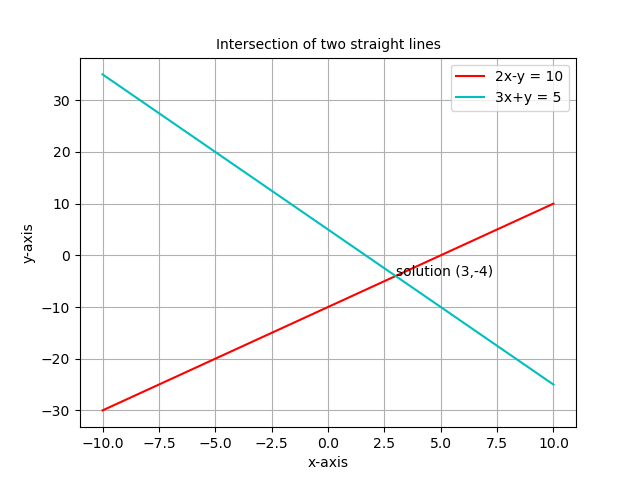
\includegraphics[width=\columnwidth]{solutions/aug/2/14/Figures/plot.png}
%          \caption{Plot of the line}
% \end{figure}

\item $\begin{alignedat}[t]{2}
2x-y&=5 
\\
x+y&=4 
\end{alignedat}$
\item Evaluate the determinant
$\begin{vmatrix}0&a&-b\\-a&0&-c\\b&c&0\end{vmatrix}=0$
\\
Find the inverse and QR decomposition of the following.
  \item \myvec{2 &1\\1 &1}\\
  \item\myvec{1 &3\\2 &7}\\
  \item\myvec{2 &3\\5 &7}\\
  \item\myvec{2 &1\\7 &4}\\
  \item \myvec{2 &5\\1 &3}\\
  \item \myvec{3 &1\\5 &2}\\
  \item \myvec{4 &5\\3 &4}\\
  \item \myvec{3 &10\\2 &7}\\
  \item \myvec{3 &-1\\-4 &2}\\
  \item \myvec{2 &-6\\1 &-2}\\
  \item \myvec{6 &-3\\-2 &1}\\
  \item \myvec{2 &-3\\-1 &2}\\
  \item \myvec{2 &1\\4 &2}\\
\item Find the QR decomposition of 
\begin{align}
\vec{A}=\myvec{8&5\\3&2} \label{eq:solutions/decomp/2/29/eq:1}
\end{align}
%%
%
\item Find the QR decomposition of 
\begin{align}
\vec{A}=\myvec{2&5\\1&4} \label{eq:solutions/decomp/2/30/1}
\end{align}

%    \end{document}    

